\documentclass{beamer}
\usepackage[utf8]{inputenc}

\usetheme{Madrid}
\usecolortheme{default}
\usepackage{amsmath,amssymb,amsfonts,amsthm}
\usepackage{txfonts}
\usepackage{tkz-euclide}
\usepackage{listings}
\usepackage{adjustbox}
\usepackage{array}
\usepackage{tabularx}
\usepackage{gvv}
\usepackage{lmodern}
\usepackage{circuitikz}
\usepackage{tikz}
\usepackage{graphicx}
\usepackage{amsmath,amssymb,amsfonts,amsthm}
\usepackage{mathtools}

\setbeamertemplate{page number in head/foot}[totalframumber]

\usepackage{tcolorbox}
\tcbuselibrary{minted,breakable,xparse,skins}



\definecolor{bg}{gray}{0.95}
\DeclareTCBListing{mintedbox}{O{}m!O{}}{%
  breakable=true,
  listing engine=minted,
  listing only,
  minted language=#2,
  minted style=default,
  minted options={%
    linenos,
    gobble=0,
    breaklines=true,
    breakafter=,,
    fontsize=\small,
    numbersep=8pt,
    #1},
  boxsep=0pt,
  left skip=0pt,
  right skip=0pt,
  left=25pt,
  right=0pt,
  top=3pt,
  bottom=3pt,
  arc=5pt,
  leftrule=0pt,
  rightrule=0pt,
  bottomrule=2pt,
  toprule=2pt,
  colback=bg,
  colframe=orange!70,
  enhanced,
  overlay={%
    \begin{tcbclipinterior}
    \fill[orange!20!white] (frame.south west) rectangle ([xshift=20pt]frame.north west);
    \end{tcbclipinterior}},
  #3,
}
\lstset{
    language=C,
    basicstyle=\ttfamily\small,
    keywordstyle=\color{blue},
    stringstyle=\color{orange},
    commentstyle=\color{green!60!black},
    numbers=left,
    numberstyle=\tiny\color{gray},
    breaklines=true,
    showstringspaces=false,
}
%------------------------------------------------------------
%This block of code defines the information to appear in the
%Title page
\title %optional
{7.4.9}
\date{October 3,2025}
%\subtitle{A short story}

\author % (optional)
{EE25BTECH11002 - Achat Parth Kalpesh}



\begin{document}

\frame{\titlepage}

\begin{frame}{Question}
   The straight line $2x-3y=1$ divides the circular region $x^2+y^2\leq6$ into two parts.\\
If  S  is $\cbrak{ \brak{2, 3/4}, \brak{5/2, 3/4}, \brak{1/4, -1/4}, \brak{1/8, 1/4} }$  then the  number of point\brak{s} in S lying inside the smaller part is  \rule{1cm}{0.01pt}.
\end{frame}

\begin{frame}{Solution:}
Let the points be 
\begin{align}
    \vec{p_1} = \myvec{2\\ \frac{3}{4}} \quad \vec{p_2} = \myvec{\frac{5}{2}\\ \frac{3}{4}} \quad \vec{p_3} = \myvec{\frac{1}{4}\\ -\frac{1}{4}} \quad \vec{p_4} = \myvec{\frac{1}{8}\\ \frac{1}{4}}
\end{align}
The circular region is 
\begin{align}
    \vec{x}^\top \vec{x} \leq 6
\end{align}
The line is
\begin{align}
    \vec{n}^\top \vec{x} = 1\\
    \vec{n} = \myvec{2\\-3}
\end{align}
\end{frame}

\begin{frame}{Solution:}
Since the origin $\vec{0}$ lies inside the circle, checking which side of the line it belongs to:
\begin{align}
    \vec{n}^\top \vec{0} - 1 = -1 < 0
\end{align}
Thus, the smaller part of the circle is the region
\begin{align}
    R = \cbrak{\vec{x} : \vec{x}^\top \vec{x} \leq 6,  \vec{n}^\top \vec{x} - 1 > 0}
\end{align}
\end{frame}

\begin{frame}{Solution:}
For $\vec{p_1}$ 
\begin{align}
  \vec{p_1}^\top \vec{p_1} &= 4 + \frac{9}{16} = \frac{73}{16} \leq 6  \\
  \vec{n}^\top \vec{p_1} - 1 &= 4 - \frac{9}{4} - 1 = \frac{3}{4} > 0
\end{align}
For $\vec{p_2}$
\begin{align}
    \vec{p_2}^\top \vec{p_2} &= \frac{109}{16} > 6\\
    \vec{n}^\top \vec{p_2} - 1 &= 5 - \frac{9}{4} - 1 = \frac{7}{4} > 0
\end{align}
For $\vec{p_3}$
\begin{align}
\vec{p_3}^\top \vec{p_3} &= \frac{1}{8} \leq 6\\
\vec{n}^\top \vec{p_3} - 1 &= \frac{1}{2}+\frac{3}{4}-1 = \frac{1}{4} > 0
\end{align}
\end{frame}

\begin{frame}{Solution:}
For $\vec{p_4}$
\begin{align}
\vec{p_4}^\top \vec{p_4} &= \frac{5}{64} \leq 6\\
\vec{n}^\top \vec{p_4} - 1 &= \frac{1}{4} - \frac{3}{4} - 1 = -\frac{3}{2} < 0
\end{align}
Thus, the points lying in the smaller part of the circle are
\begin{align}
    \vec{p_1} = \myvec{2\\ \frac{3}{4}} \quad \vec{p_3} = \myvec{\frac{1}{4}\\ -\frac{1}{4}}
\end{align}
\end{frame}



\begin{frame}[fragile]
  \frametitle{C Code}
  \begin{lstlisting}[language=C]
#include <stdio.h>
double get_circle_radius() {
    return 2.449489742783178; // sqrt(6)
}
double line_equation(double x) {
    return (2*x - 1)/3;
}
int is_inside_circle(double x, double y) {
    return (x*x + y*y <= 6) ? 1 : 0;
}
int is_on_positive_side(double x, double y) {
    return (2*x - 3*y - 1 > 0) ? 1 : 0;
}
int is_inside_smaller_region(double x, double y) {
    return is_inside_circle(x, y) && is_on_positive_side(x, y);
}
  \end{lstlisting}
\end{frame}

\begin{frame}[fragile]
  \frametitle{Python Code}
  \begin{lstlisting}[language=Python]
import ctypes
import numpy as np
import matplotlib.pyplot as plt
formula = ctypes.CDLL("./formula.so")

# Declare argument & return types for functions (same as in C)
formula.get_circle_radius.restype = ctypes.c_double
formula.line_equation.argtypes = [ctypes.c_double]
formula.line_equation.restype = ctypes.c_double
formula.is_inside_circle.argtypes = [ctypes.c_double, ctypes.c_double]
formula.is_inside_circle.restype = ctypes.c_int
formula.is_on_positive_side.argtypes = [ctypes.c_double, ctypes.c_double]
formula.is_on_positive_side.restype = ctypes.c_int
formula.is_inside_smaller_region.argtypes = [ctypes.c_double, ctypes.c_double]
formula.is_inside_smaller_region.restype = ctypes.c_int
  \end{lstlisting}
\end{frame}

\begin{frame}[fragile]
  \frametitle{Python Code}
  \begin{lstlisting}[language=Python]
# Circle parameters: x^2 + y^2 = 6
r = np.sqrt(6)

# Line: 2x - 3y = 1 => y = (2x - 1)/3
x_line = np.linspace(-3, 3, 400)
y_line = (2*x_line - 1) / 3

# Points
points = {
    "$p_1$(2, 3/4)": (2, 0.75),
    "$p_3$(1/4, -1/4)": (0.25, -0.25),
    "$p_4$(1/8, 1/4)": (0.125, 0.25)
}
point = {
    "$p_2$(5/2 ,3/4)": (2.5, 0.75),
}
  \end{lstlisting}
\end{frame}
\begin{frame}[fragile]
  \frametitle{Python Code}
  \begin{lstlisting}[language=Python]
# Circle boundary
theta = np.linspace(0, 2*np.pi, 500)
x_circle = r * np.cos(theta)
y_circle = r * np.sin(theta)
plt.figure(figsize=(7,7))
plt.plot(x_circle, y_circle, 'b')
plt.text(r*np.cos(np.pi/4), r*np.sin(np.pi/4), "x² + y² = 6", color='b', fontsize=10)
# Line
plt.plot(x_line, y_line, 'r')
plt.text(-2.5, -2.5, "2x - 3y = 1", color='r', fontsize=10)

# Shaded region (smaller part)
xx, yy = np.meshgrid(np.linspace(-r, r, 400), np.linspace(-r, r, 400))
mask_circle = xx**2 + yy**2 <= 6
mask_line = 2*xx - 3*yy - 1 > 0
mask = mask_circle & mask_line
  \end{lstlisting}
\end{frame}

\begin{frame}[fragile]
  \frametitle{Python Code}
  \begin{lstlisting}[language=Python]
plt.contourf(xx, yy, mask, levels=[0.5, 1], colors=['#ffcccc'], alpha=0.5)
plt.text(0, -2, "Smaller region", color='darkred', fontsize=10)

# Plot points
for label, (x, y) in points.items():
    plt.scatter(x, y, s=70)
    plt.text(x-0.5, y-0.35, label, fontsize=9)

for label, (x, y) in point.items():
    plt.scatter(x, y, s=70)
    plt.text(x-0.3, y-0.3, label, fontsize=9)

  \end{lstlisting}
\end{frame}
\begin{frame}[fragile]
  \frametitle{Python Code}
  \begin{lstlisting}[language=Python]

# Formatting
plt.gca().set_aspect('equal', adjustable='box')
plt.axhline(0, color='black', linewidth=0.5)
plt.axvline(0, color='black', linewidth=0.5)
plt.xlim(-3,3)
plt.ylim(-3,3)
plt.grid(True)
plt.title("Circle cut by the Line")
plt.show()
  \end{lstlisting}
\end{frame}

\begin{frame}{Plot}
  \begin{figure}
    \centering
    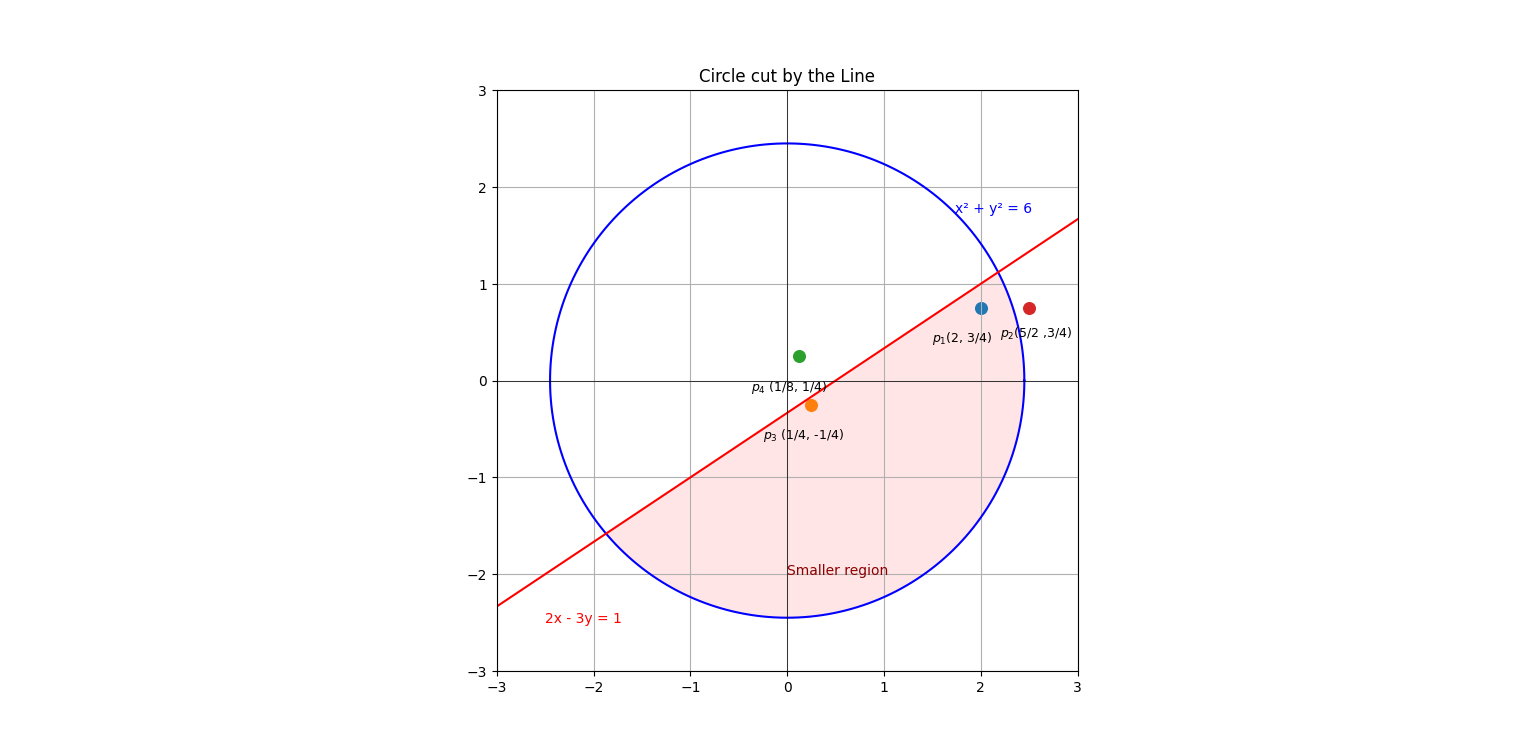
\includegraphics[width=\textwidth]{../figs/figure_py.png}
    \caption{Visualization of the solution.}
    \label{fig:final_plot}
  \end{figure}
\end{frame}

\end{document}
